\documentclass[10pt,a4paper]{article}
\usepackage{ikps,ansform}
\usepackage{lipsum}
\usepackage{kotex}
\usepackage[left=1in, right=1in, top=1in, bottom=1in]{geometry}
\usepackage{indentfirst}
\usepackage{listings}
\usepackage[bookmarks=true,pdfborder={0 0 0}]{hyperref}
\usepackage{graphicx}
\usepackage{setspace}

\renewcommand{\indent}{\hspace*{10pt}}
\renewenvironment{abstract}{
	\begin{center}
		{\noindent\textbf{\large요 약}}
	\end{center}\indent}

\renewcommand{\contentsname}{\center차\hspace*{12pt}례}
\renewcommand{\lstlistingname}{소스코드}
\renewcommand{\lstlistlistingname}{\center소스코드 목차}
\renewcommand{\figurename}{그림}
\renewcommand{\refname}{참고문헌}

\lstset{frame=tb,
	language=C++,
	aboveskip=3mm,
	belowskip=3mm,
	showstringspaces=false,
	basicstyle=\normalsize,  % 2019 소스 글자크기 조정 함
	numbers=left,
	stepnumber=5,  % 점프 사이즈
	showstringspaces=false,
	tabsize=1,
	breaklines=true,
	breakatwhitespace=false,
	columns=flexible,
	basicstyle={\normalsize\ttfamily},
	numberstyle=\small\color{blue},
	keywordstyle=\color{blue},
	commentstyle=\color{teal},
	stringstyle=\color{magenta},
	breaklines=true,
	breakatwhitespace=true,
	tabsize=3
}

\title{\textbf{분할정복법을 이용한 기하학적 문제 해결 방법}}
\author{김현수(201424442)\\[3mm]부산대학교 공과대학 정보컴퓨터공학전공\\[3mm]\textit{alcatraz@pusan.ac.kr}}
\date{2020년 04월 20일}

\begin{document}
\maketitle
\tableofcontents
\begin{spacing}{1.6}
\section{서론}
  분할정복 기법(Devide and Conquer)란, 어떠한 문제를 일정한 크기의 문제로 분할하여 답을 구한 후, 답들을 종합하여 전체 문제의 답을 구하는 방법이다. 분할정복 기법은 문제를 분할하면, 계산량이 적어지는 문제에 적용할 수 있다. 2절에서는 주어진 선분 중에서 다른 선분과 만나지 않는 선분만 추려낸 후 남은 선분의 최소 거리를 구하는 문제에 대하여 이야기하고, 3절에서는 중첩되는 직사각형이 이루는 윤곽을 계산하는 문제에 대하여 논한다.
  
\section{PA01-1}
  PA01-1 문제는 주어진 선분 중에서 다른 선분과 만나는 선분을 제거하고, 남은 선분들 사이의 최소거리를 구하려는 문제이다. 이 문제는 (1) 다른 선분과 만나는 선분을 제거하는 것과 (2) (1)에서 제거하고 남은 선분들에 대하여 최소 거리를 구하는 것으로 나눈다. 
  
  이후 (1)과 (2)를 분할정복 기법을 이용하여 각각 푼다. 이를 위해서 Merge Sort에서의 발상을 적용하였다. 2.1은 (1)을 푸는 방법에 대한 설명이고, 2.2에서는 (2)를 푸는 방법에 대하여 설명한 후 2.3에서 이 문제를 풀기 위한 시간복잡도를 분석한다. 
  
\subsection{서로 만나는 선분을 제거하는 방법}
\subsubsection{두 직선의 위치관계와 벡터의 외적}
  이 절에서는 입력된 자료를 통하여 서로 만나는 선분을 제거하는 방법에 대하여 살핀다. 그림 \ref{fig1}은 두 선분AB, CD가 서로 교차하는 경우에 대하여 나타낸 것이다. 
  \begin{figure}
  	\centering
  	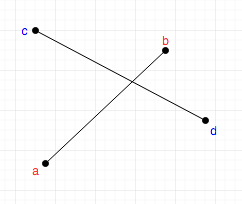
\includegraphics[scale=1]{Fig1.png}
  	\caption{교차하고 있는 선분 AB, CD}
  	\label{fig1}
  \end{figure}

  \begin{figure}
	\centering
	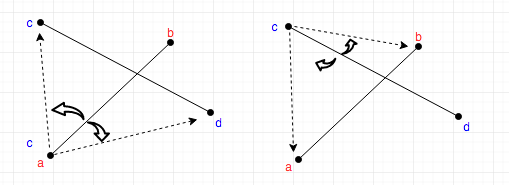
\includegraphics[scale=1]{Fig2.png}
	\caption{교차하고 있는 선분 AB, CD의 위치관계 } 
	\label{fig2}
  \end{figure}

    그림 \ref{fig2}는 선분 AB와 선분 CD가 서로 교차할 때, 각 점이 생성할 수 있는 벡터와 선분간의 위치관계를 살핀 것이다. $\angle{\mathrm{BAC}}$와 $\angle{\mathrm{BAD}}$는 $\ovr{\mathrm{AB}}$를 시초선으로 할 때, 서로 반대 방향의 동경이 생성한 각이므로 삼각함수의 성질에 의하여 $\vec{\mathrm{BA}} \times \vec{\mathrm{CA}}$의 값과 $\vec{\mathrm{BA}} \times \vec{\mathrm{DA}}$의 곱은 음수가 된다. 이는 선분 CD와 점 A, B에 대하여도 동일하게 적용된다. \footnote{두 벡터 $\vec{a}$,$\vec{b}$가 있고, 두 벡터가 이루는 최소의 각의 크기를 $\theta$라 하면, $\vec{a} \times \vec{b} = |a||b|\sin{\theta}$}
    
    그러므로, 벡터의 외적값에 따른 직선의 위치관계를 확인하기 위하여 각 점 A, B, C, D에 대하여 다음의 값을 구한다. 
    \begin{itemize}
    	\item $\vec{\mathrm{BA}} \times \vec{\mathrm{CA}}$
    	\item $\vec{\mathrm{BA}} \times \vec{\mathrm{DA}}$
    	\item $\vec{\mathrm{DC}} \times \vec{\mathrm{AC}}$
    	\item $\vec{\mathrm{BC}} \times \vec{\mathrm{DC}}$
    \end{itemize}

    위에서 서술한 값들 중에서 $\vec{\mathrm{BA}} \times \vec{\mathrm{CA}}$와 $\vec{\mathrm{BA}} \times \vec{\mathrm{DA}}$의 곱을 $\alpha$라고 하고, $\vec{\mathrm{DC}} \times \vec{\mathrm{AC}}$ 과 $\vec{\mathrm{BC}} \times \vec{\mathrm{DC}}$의 곱을 $\beta$라고 하자. 만약, 선분 AB와 선분 BC가 그림 2와 깉은 위치관계가 있다면 수식 \ref{eq1} 의 관계가 성립한다. 
    \begin{equation}
    \alpha \times \beta \leq 0
    \label{eq1}
    \end{equation}
    
   	특히, $\alpha \times \beta = 0$이면, 선분 AB와 선분 BC는 한 직선 $l$에 속하거나, 적어도 하나의 점이 일치하게 되고, 이 경우는 해답에서 제외하여야 한다.
\subsubsection{풀이 방법}
  2.1.1에서 살펴본 방법을 분할정복 기법을 이용하여 동작하도록 한다. 이때, 입력받은 데이터를 각 점의 $x$좌표와 $y$좌표의 크기에 따라 정렬하면, 좌표평면에 점이 놓이는 순서대로 정렬되므로, 좌표평면을 일정한 구간으로 분할하는 것과 같은 결과를 만든다. 
  
  풀이를 위하여 입력과 출력을 정의한다.
  \begin{center}
  	\textbf{(입력)} 정수형 순서쌍의 순서쌍 $Line = (x,y),(x,y)$ 의 배열 \textit{linearr} \\
  	\textbf{(출력)} 정수형 순서쌍의 순서쌍  $Line = (x,y),(x,y)$ 의 배열 \textit{linearr$\_$res}
  \end{center}

  이후 다음의 과정을 거친다. 
  \begin{enumerate}
  	\item 입력을 절반으로 나눈다.
  	\item 절반으로 나눈 부분에 대하여 2.1.1을 각각 수행한다.
  	\item 2의 과정으로부터 나오는 결과를 Merge한다.
  \end{enumerate}

\subsection{선분간의 거리의 최솟값을 구하는 방법}
  선분간의 거리는 각 선분의 양 끝검으루부터 다른 선분까지의 거리 중 최솟값으로 한다. 이 때, 선분간의 거리는 구하고자 하는 선분이 속한 직선의 방정식으로부터 유도할 수 있다. 이를 위해서는 2.1에 필요한 정보를 입력받으면서 직선의 방정식에 필요한 계수를 계산한다. 
  
  두 점 $A(x_1,y_1), B(x_2, y_2)$을 지나는 직선 $l$의 방정식은 수식 \ref{eq2}와 같이 계산할 수 있다. 
  	\begin{equation}
  	\begin{aligned}
 	 l : & (y-y_1) = \dfrac{y_2-y_1}{x_2-x_1} (x-x_1) \\
  		  & (y_2-y_1)(x-x_1)-(x_2-x_1)(y-y_1)\\
  	 	 & = (y_2-y_1)x - (x_2-x_1)y + \lbrace(x_2-x_1)y_1 - (y_2-y_1)x_1\rbrace\\
  	  	& = ax+by+c = 0
  \end{aligned}
	\label{eq2}  
	\end{equation}
	
	수식 \ref{eq2}와 같은 계산을 통하여 얻은 계수 $a,b,c$와 다른 선분 위의 한 점 $(\alpha,\beta)$ 사이의 거리는 수식 \ref{eq3}과 같다. 
	\begin{equation}
	\frac{|a\alpha+b\beta+c|}{\sqrt{a^2+b^2}}
	\label{eq3}
	\end{equation}

  이러한 계산을 2.1의 결과로 도출된 출력을 입력으로 하여 2.1과 같은 방법으로 계산하여 최솟값을 구하면 된다. 
  
\subsection{시간복잡도 분석}
  2.1.1, 2.1.2의 방법에 대한 시간복잡도를 살핀다. 2.1.1의 시간복잡도를 $T_{2.1.1}(n)$이라 하고, 2.1.1의 입력의 절반을 $left = \lfloor \dfrac{n}{2} \rfloor $, 나머지 절반을 $right = \lceil \dfrac{n}{2} \rceil$이라 하다. 
  
  만일 n이 2의 거듭제곱이라 하면, 
  \begin{equation*}
  \begin{aligned}
  T_{2.1.1}(n) &= T_{2.1.1}(left) + T_{2.1.1}(right) + (mergetime)\\
  mergetime &= left + right -1 \\ 
  left  &= \lfloor \dfrac{n}{2} \rfloor = \dfrac{n}{2} \\
  right &= n - left = \lceil \dfrac{n}{2} \rceil= \dfrac{n}{2} \\
  left + right &= n = 2^k (k \in \mathbb{Z}^{+})
  \end{aligned}
  \end{equation*}
  
  이 되어 
  \begin{equation*}
  \begin{aligned}
  T_{2.1.1}(n) &= 2T_{2.1.1}(\dfrac{n}{2})) + (n-1)\\
  \end{aligned}
  \end{equation*}
  
  이 되며, $n=1$인 때는 교차유무를 확인할 수 없으므로 $T_{2.1.1}(1) = 0$이다. 따라서, 
    \begin{equation*}
  \begin{aligned}
  T_{2.1.1}(n) &= 2T_{2.1.1}(\dfrac{n}{2})) + (n-1)\\
   &= 2^{k}T_{2.1.1}(1) + kn - \sum_{i=0}^{k-1}{2^i} \\
   &= kn+1-2^k = n\lg{n} - (n-1) ( \because n = 2^k ,k \in \mathbb{Z}^{+} )\\
   &\in \Theta(n\lg{n})
  \end{aligned}
  \end{equation*}
  이다. 
  
  2.2.2의 방법은 2.1.1과 동일하므로 $T_{2.2.2}(n) \in \Theta(n\lg{n})$이어서 $n$개의 선분에 대하여 PA01-1을 해결하는데 필요한 시간의 복잡도는 $T(n) = 2 \times \Theta(n\lg{n}) \in \Theta(n\lg{n}) $이다.
  
\section{PA01-2}
  PA01-2는 2.1과 동일한 발상을 이용한다. 다만, 사각형이 겹치는 구간이 있는지의 여부를 분할정복기법을 통하여 살피면 된다. 시간복잡도는 2.1과 동일하게 $T(n) = 2 \times \Theta(n\lg{n}) \in \Theta(n\lg{n}) $이다. 
 
\end{spacing}
\end{document}
